\section{Algorithm}
We apply the component-wise boosting algorithm \ref{algo:fhtboost} with loss function $\rho(\mu,\y0)=-\log\loss{y_0,\mu}$. We differentiate the loss function with respect to these two and get .... For more details on the derivation, see \ref{appendix}. \todo{Maybe use $b$ instead of $y_0$, to not get subscript chaos?}

\begin{algorithm}
\caption{FHT Boost with twodimensional loss function}
\label{algo:fhtboost}
\begin{enumerate}
    \item Initialize the $n$-dimensional vectors $\hat{y}_0^{[0]},\hat{\mu}^{[0]}$ with the maximum likelihood estimates as offset values, i.e., $\hat{y}_0^{[0]}, \hat{\mu}^{[0]}=\argmin_{y_0,\mu}\rho(\cdot,\cdot)$.
    \item For both components of the loss function, we specify linear base learners. In particular, a component-wise base learner which can be used for each of the $p$ variables used in $\X$ corresponding to $y_0$ and the $d$ variables in $\Z$ corresponding to $\mu$. Like earlier, the base learner takes one input variable and has one output variable.
    \item Set $m=0$ and $\nu=0.1$.
    \item Increase $m$ by 1.
    \begin{enumerate}
        \item If $m>m_{\text{stop},y_0}$, proceed to step 4 e). If not, compute the negative partial derivative $-\frac{\partial\rho}{\partial y_0}$ and evaluate at $\hat{f}^{[m-1]}(X_i,Z_i)=\left(\hat{y}_0^{[m-1]}(X_i),\hat{\mu}^{[m-1]}(Z_i)\right)_{i=1,\ldots,n}$. This yields the negative gradient vector $U_{y_0}^{[m-1]}=\left(U_{i,y_0}^{[m-1]}\right)_{i=1,\ldots,n}:=\left(-\frac{\partial}{\partial y_0}\rho\left(Y_i,\hat{f}^{[m-1]}(X_i,Z_i)\right)\right)_{i=1,\ldots,n}$.
        \item Fit the negative gradient vector $U_{y_0}^{[m-1]}$ to each of the $p$ components of $\X$ separately (i.e. to each predictor variable) using the base learners specified in step 2. This yields $p$ vectors of predicted values, where each vector is an estimate of the negative gradient vector $U_{y_0}^{[m-1]}$.
        \item Select the component of $\X$ which best fits $U_{y_0}{[m-1]}$ according to $R^2$. Set $\hat{U}_{y_0}^{[m-1]}$ equal to the fitted values of the corresponding best model fitted in the previous step.
        \item Update $\hat{y}_0^{[m-1]}\gets\hat{y}_0^{[m-1]}+\nu\hat{U}_{y_0}^{[m-1]}$.
        \item If $m>m_{\text{stop},\mu}$, proceed to step 4 j). If not, compute the negative partial derivative $-\frac{\partial\rho}{\partial \mu}$ and evaluate at $\hat{f}^{[m-1]}(X_i,Z_i)=\left(\hat{y}_0^{[m-1]}(X_i),\hat{\mu}^{[m-1]}(Z_i)\right)_{i=1,\ldots,n}$. This yields the negative gradient vector $U_{\mu}^{[m-1]}=\left(U_{i,\mu}^{[m-1]}\right)_{i=1,\ldots,n}:=\left(-\frac{\partial}{\partial \mu}\rho\left(Y_i,\hat{f}^{[m-1]}(X_i,Z_i)\right)\right)_{i=1,\ldots,n}$.
        \item Fit the negative gradient vector $U_{\mu}^{[m-1]}$ to each of the $p$ components of $\Z$ separately (i.e. to each predictor variable) using the base learners specified in step 2. This yields $d$ vectors of predicted values, where each vector is an estimate of the negative gradient vector $U_{\mu}^{[m-1]}$.
        \item Select the component of $\Z$ which best fits $U_{\mu}{[m-1]}$ according to $R^2$. Set $\hat{U}_{\mu}^{[m-1]}$ equal to the fitted values of the corresponding best model fitted in the previous step.
        \item Update $\hat{\mu}^{[m-1]}\gets\hat{\mu}^{[m-1]}+\nu\hat{U}_{\mu}^{[m-1]}$.
        \item Update $\hat{f}^{[m]}\gets\hat{f}^{[m-1]}$.
        \item If $m>\max(m_{\text{stop},y_0},m_{\text{stop},\mu})$, go to step 5. If not, repeat step 4.
    \end{enumerate}
    \item Return $\hat{f}^{[m]}$.
\end{enumerate}
\end{algorithm}
We might call this cyclical boosting.

\subsection{Boost in same}
Another way to do this is to only boost one component in each iteration. The component might be corresponding to $X$, or it might be corresponding to $Z$.


% First tried cyclical boosting.
% Then tried non-cyclical, with comparing RSS. Doesn't work; not on the same scale.
% Then tried using non-cyclical, comparing instead the loss function instead of rss.

\subsection{Derivatives not on same scale}
Pass.

\subsection{Changing the intercept in each iteration}
Another way to do this is to only boost one component in each iteration. The component might be corresponding to $X$, or it might be corresponding to $Z$.


\section{Simulation experiments}
In this section, I will discuss how I tried validating the boosting method I have developed. While working with implementing the algorithm, to see if it worked, I first used an example with low dimensions. In low dimensions, it's feasible to find the joint maximum likelihood numerically. After confirming the method works as it should, we can go to more complicated examples.

\subsection{Small example}
Let parameter vectors be two dense $\bbeta=(2,0.1,0.2)$ and $\bgamma=(-1, -0.1, 0.1)$. Let $X$ and $Z$ be such and such, drawn from a beta distribution.
We simulate data using Algorithm \ref{algo:FHT-sim}, with the censoring time $W$ being drawn from a distribution $\exp(0.1)$. The resulting survival times have the following Kaplan-Meier plot.
\begin{figure}[H]\centering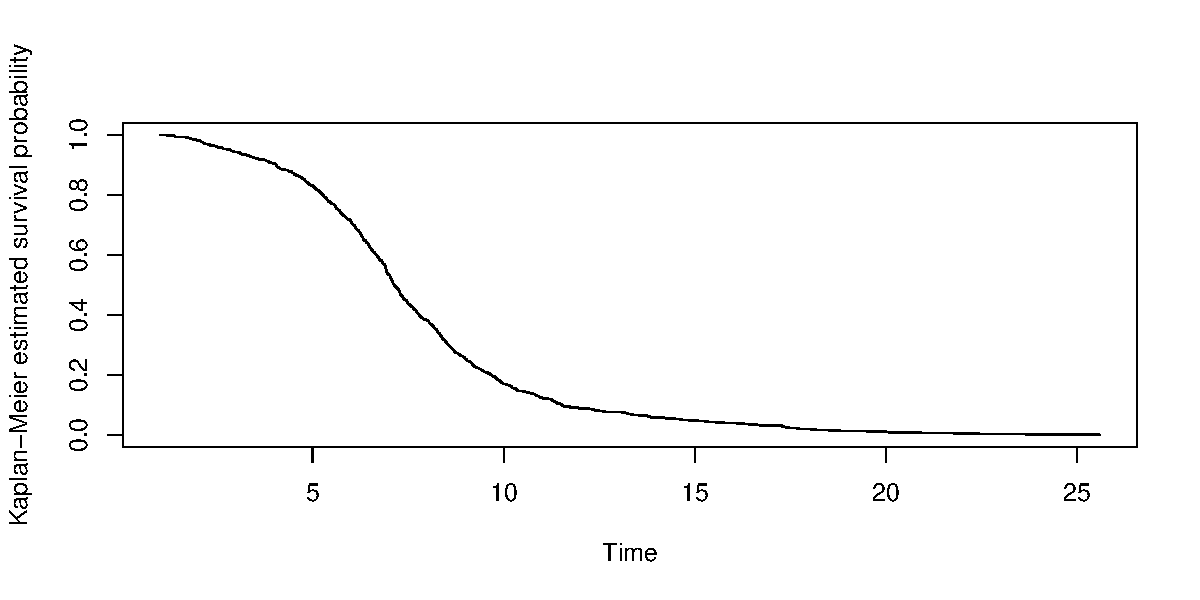
\includegraphics[scale=0.4]{figures/case1.pdf}\end{figure}
We use cross validation to find a suitable iteration number $\mstop$, and find it to be 28. We then run our algorithm with that number of iterations. Below is a plot of the negative log likelihood of the data (in-sample loss) as a function of iteration number.
\begin{figure}[H]\centering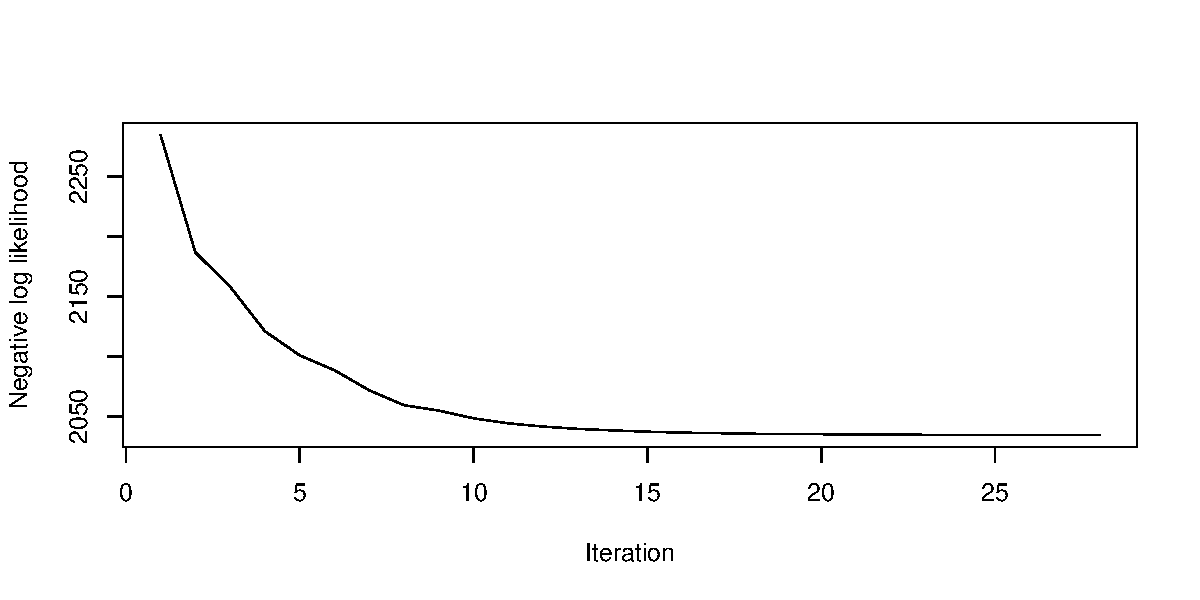
\includegraphics[scale=0.4]{figures/case1_loglik.pdf}\end{figure}
The final $\hat{\bbeta}$ is $(1.968, 0.103, 0.180)$, and the final $\hat{\bgamma}$ is $(-0.964, -0.082, 0.062)$. The parameters found by numerically maximizing the joint maximum likelihood are also included. Summarized in the table below.

\begin{tabular}{lrr}
    parameter  & true & estimated \\
    $\beta_0$  &  2.0 &     1.968 \\
    $\beta_1$  &  0.1 &     0.103 \\
    $\beta_2$  &  0.2 &     0.180 \\
    $\gamma_0$ & -1.0 &    -0.964 \\
    $\gamma_1$ & -0.1 &    -0.082 \\
    $\gamma_2$ &  0.1 &     0.062 \\
\end{tabular}

As we can see, our boosting method recovers the original parameters quite well. This is of course with data coming from the exact same kind of model.

\subsection{Large example with uncorrelated matrices}
Here, $N$ is 1000. We let $\bbeta$ be a large vector of size $p=10001$, and $\bgamma$ be a small vector of size $d=16$. We imagine $X$, corresponding to $\bbeta$, be gene expressions, whereas $Z$, corresponding to $\bgamma$ be clinical measurements. Specifically, we set the intercept term in $\bbeta$ to be 2.0, and the first 35 elements to be 0.1. We set the rest to be 0. For $\bgamma$, we set the intercept term to be -1, and in similar fashion, let the first 5 elements have a non-zero value of -0.1. Here also we set the remaining 10 elements to be 0.
We also here draw $X$ and $Z$ from a beta distribution. The resulting survival times have the following Kaplan-Meier plot.
\begin{figure}[H]\centering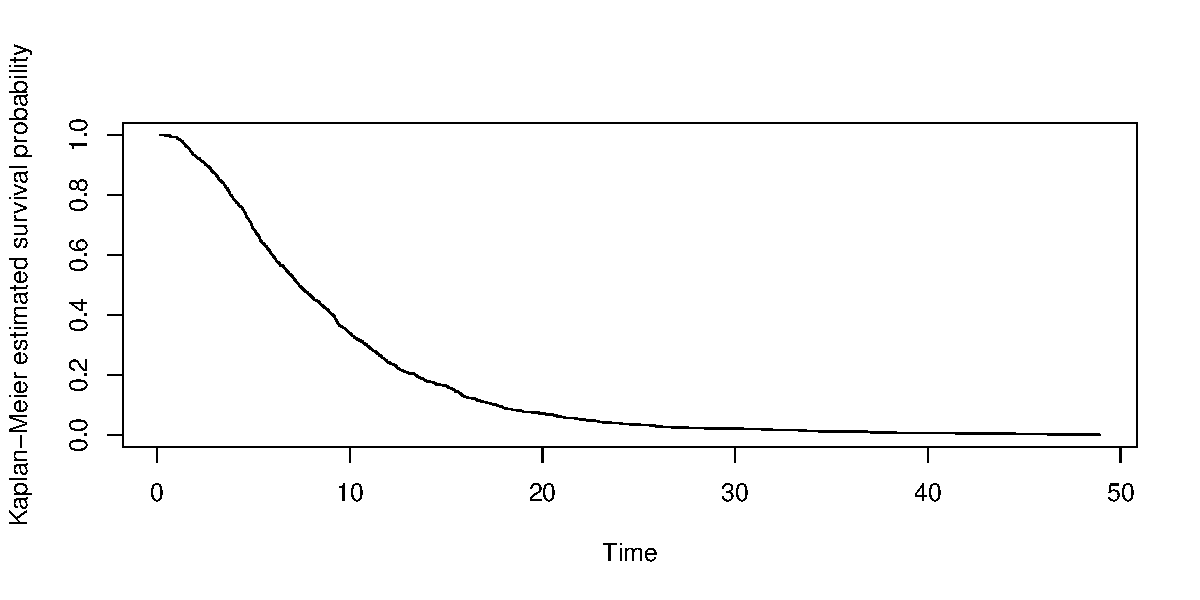
\includegraphics[scale=0.4]{figures/case2.pdf}\end{figure}
We use cross validation to find a suitable iteration number $\mstop$, and find it to be 80. We then run our algorithm with that number of iterations. We find that elements ... are selected. They are 

\subsection{Large example with correlated matrices}
Here, $N$ is 1000. We let $\bbeta$ be a large vector of size $p=10001$, and $\bgamma$ be a small vector of size $d=16$. We imagine $X$, corresponding to $\bbeta$, be gene expressions, whereas $Z$, corresponding to $\bgamma$ be clinical measurements. Specifically, we set the intercept term in $\bbeta$ to be 2.0, and the first 35 elements to be 0.1. We set the rest to be 0. For $\bgamma$, we set the intercept term to be -1, and in similar fashion, let the first 5 elements have a non-zero value of -0.1. Here also we set the remaining 10 elements to be 0.
